% !TeX program = xelatex
\documentclass[10pt,aspectratio=169]{beamer}
\geometry{paperwidth=180mm,paperheight=101.25mm}
\usepackage{fontspec}
\setsansfont{texgyreheros}[Extension=.otf,UprightFont=*-regular,BoldFont=*-bold,ItalicFont=*-italic,BoldItalicFont=*-bolditalic]
\setmonofont[Scale=0.88]{lmmono10-regular.otf}
\usepackage{booktabs,tabularx,array,tikz}
\usetikzlibrary{arrows.meta,positioning,calc}
\definecolor{Navy}{HTML}{17324D}
\definecolor{Teal}{HTML}{007F82}
\definecolor{Blue}{HTML}{4178B5}
\definecolor{Amber}{HTML}{A86B17}
\definecolor{Slate}{HTML}{586878}
\definecolor{Pale}{HTML}{F0F4F7}
\setbeamercolor{normal text}{fg=Navy,bg=white}
\setbeamercolor{structure}{fg=Teal}
\setbeamercolor{frametitle}{fg=Navy}
\setbeamerfont{frametitle}{size=\Large,series=\bfseries}
\setbeamercolor{block title}{fg=Navy,bg=Pale}
\setbeamercolor{block body}{fg=Navy,bg=Pale}
\setbeamerfont{block title}{size=\normalsize,series=\bfseries}
\setbeamertemplate{navigation symbols}{}
\setbeamersize{text margin left=7mm,text margin right=7mm}
\setbeamertemplate{headline}{\vspace{2mm}\hspace{7mm}{\color{Teal}\fontsize{7.5}{9}\selectfont\bfseries TRACE-Q\quad /\quad\insertsectionnumber\enspace\MakeUppercase{\insertsectionhead}}\vspace{1mm}}
\setbeamertemplate{frametitle}{\vspace{0mm}\insertframetitle\par\vspace{1mm}}
\setbeamertemplate{footline}{\hspace{7mm}{\color{Slate}\fontsize{6.8}{8}\selectfont FINAL HUMAN REVIEW v2.4.1\quad |\quad OCTOBER 22, 2026}\hfill{\color{Slate}\fontsize{7.5}{9}\selectfont\insertframenumber\,/\,\inserttotalframenumber}\hspace{7mm}\vspace{2mm}}
\setbeamertemplate{itemize item}{\color{Teal}\small\textbullet}
\setlength{\tabcolsep}{5pt}
\renewcommand{\arraystretch}{1.16}
\newcolumntype{Y}{>{\raggedright\arraybackslash}X}
\newcommand{\code}[1]{{\ttfamily\fontsize{8}{9.5}\selectfont\detokenize{#1}}}
\newcommand{\src}[1]{\par\vfill{\color{Slate}\fontsize{6.5}{8}\selectfont #1\par}}
\newcommand{\takeaway}[1]{\par\medskip{\color{Teal}\bfseries #1}\par}
\newcommand{\smalltext}{\fontsize{8.5}{10.4}\selectfont}
\hypersetup{pdftitle={TRACE-Q: Review Codebook and Changes in Confirmed Statistical Findings},pdfauthor={},pdfsubject={Three-section presentation based on the October 22, 2026 manuscript and final v2.4.1 human review workbooks}}
\begin{document}

\section{Paper and study design}
\begin{frame}[t]{TRACE-Q: from review flags to statistical findings}
\vspace{1mm}
{\large An exploratory toolkit for evidence-grounded review\\of quantitative research reporting}\par
\vspace{4mm}
\begin{columns}[T,onlytextwidth]
\column{.31\textwidth}
{\color{Blue}\fontsize{30}{32}\selectfont\bfseries 139}\par
\textbf{Confirmed all}\par
\small Statistical findings of any\newline substantive importance
\column{.31\textwidth}
{\color{Teal}\fontsize{30}{32}\selectfont\bfseries 37}\par
\textbf{Confirmed substantive}\par
\small Subset with potential to affect\newline interpretation or data use
\column{.31\textwidth}
{\color{Navy}\fontsize{30}{32}\selectfont\bfseries 44}\par
\textbf{Trial packages}\par
\small 19 earlier and 25 later reports\newline from selected JAMA trials
\end{columns}
\vspace{5mm}
\begin{tabularx}{\linewidth}{@{}rY@{}}
\textcolor{Teal}{\textbf{01}} & Paper and study design: what TRACE-Q checks and what was sampled.\\
\textcolor{Teal}{\textbf{02}} & Review codebook: how a candidate becomes an eligible finding.\\
\textcolor{Teal}{\textbf{03}} & Statistical results: confirmed all versus confirmed substantive over time.
\end{tabularx}
\src{Source: TRACE-Q draft and supplement, October 22, 2026; four completed human review workbooks. Here, ``confirmed all'' refers specifically to statistical findings with original report-only relationships.}
\end{frame}

\begin{frame}[t]{Evidence stays linked through checking and review}
\begin{columns}[T,onlytextwidth]
\column{.47\textwidth}
\centering
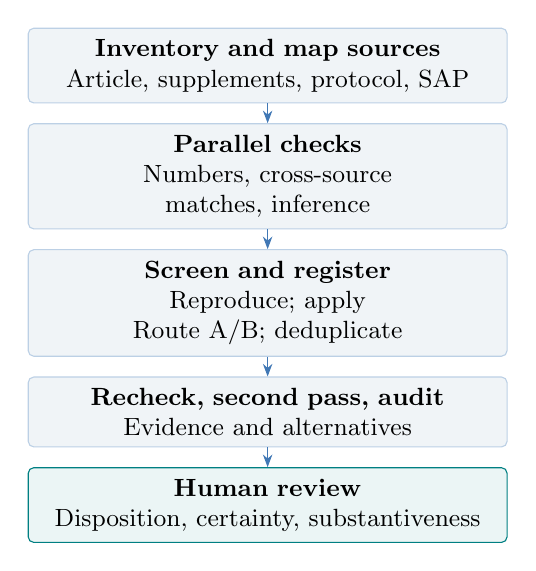
\begin{tikzpicture}[font=\small,node distance=2.5mm,
 box/.style={draw=Blue!35,fill=Pale,rounded corners=2pt,text width=5.8cm,align=center,inner sep=4pt},
 arr/.style={-{Stealth[length=1.6mm]},draw=Blue}]
\node[box] (map) {\textbf{Inventory and map sources}\\Article, supplements, protocol, SAP};
\node[box,below=of map] (check) {\textbf{Parallel checks}\\Numbers, cross-source matches, inference};
\node[box,below=of check] (screen) {\textbf{Screen and register}\\Reproduce; apply Route A/B; deduplicate};
\node[box,below=of screen] (recheck) {\textbf{Recheck, second pass, audit}\\Evidence and alternatives};
\node[box,below=of recheck,fill=Teal!8,draw=Teal] (human) {\textbf{Human review}\\Disposition, certainty, substantiveness};
\foreach \a/\b in {map/check,check/screen,screen/recheck,recheck/human}\draw[arr](\a)--(\b);
\end{tikzpicture}
\column{.49\textwidth}
\small
\textbf{Why the workflow exists}\par
Reconcile numbers spread across documents while preserving source locations and checking history.
\medskip\par
\textbf{Route A: specified discrepancies}\par
Examples include interval--test incompatibility, irreconcilable counts, interpretation-changing slips, or specified planned-analysis changes/omissions.
\medskip\par
\textbf{Route B: consequential ambiguity}\par
An in-scope concern cannot be immediately resolved and could affect a named result's interpretation or extraction.
\medskip\par
\textcolor{Teal}{\textbf{A registered flag still requires human judgment.}} Coverage and rechecking do not establish detection accuracy.
\end{columns}
\src{Source: manuscript, TRACE-Q Framework. Workflow 1.6.2; model gpt-6.1-sol. SAP = statistical analysis plan. The second pass sees earlier outputs and is not blinded replication.}
\end{frame}

\begin{frame}[t]{The comparison uses 44 selected trial packages}
\begin{columns}[T,onlytextwidth]
\column{.59\textwidth}
\small
\begin{tabular}{@{}lrrrr@{}}
\toprule
Year & Papers & PDF pages & Flags & Retained\\\midrule
2018 & 10 & 1,070 & 115 & 107\\
2019 & 9 & 994 & 79 & 76\\
2024 & 10 & 1,097 & 113 & 107\\
2025 & 15 & 2,398 & 133 & 123\\\midrule
\textbf{Total} & \textbf{44} & \textbf{5,559} & \textbf{440} & \textbf{413}\\\bottomrule
\end{tabular}
\medskip\par
188 PDFs plus one supplementary Excel worksheet. Plans may be embedded in supplements.
\medskip\par
\textbf{Period denominators}\par
2018--2019: \textbf{19 papers}\quad 2024--2025: \textbf{25 papers}
\column{.36\textwidth}
\begin{block}{Human review}
\small
413 retained; 27 excluded.\\
All 440 entries completed; no deferred dispositions.\\[2mm]
One recorded reviewer: \code{R_Bulun}. No independent second ratings.
\end{block}
\small
Availability sample of primary randomized JAMA trials in the selected publication years. No complete journal screening log.
\end{columns}
\takeaway{Retention includes descriptive differences and uncertain findings.}
\src{Source: manuscript, Application and Results; analysis/year\_summary.csv. Cohort follows recorded online-first year, which can differ from the DOI year. Retention is not an accuracy estimate.}
\end{frame}

\section{Review codebook in detail}
\begin{frame}[t]{Common fields establish a traceable human decision}
\smalltext
\begin{tabularx}{\linewidth}{@{}p{2.9cm}Y@{}}
\toprule
Field (column) & Operational rule in codebook v2.4.1\\\midrule
Identity and evidence (A--C) & Preserve the candidate key; the title is a flag, not a verdict. Open the original file and PDF page named in the source location.\\
Review domain (E) & Choose the assessment branch first. The AI suggestion is editable; the original document relationship code stays frozen.\\
Disposition (D) & \code{retain}: keep for applicable summaries; \code{exclude}: remove after assessment; \code{discuss}: considered but deferred. A blank means unanswered.\\
Completion (F) & Use \code{no} while drafting and \code{primary_done} after manual review. Reset to \code{no} before editing a completed row; then review and complete again.\\
Validation hint (G) & Calculated \code{PRIMARY READY} means valid entry plus manual completion, including a deferred \code{discuss} decision. It does not certify scientific accuracy.\\
Notes (R) & Optional English context; no inherited answers. Clear obsolete literal answers when changing branches.\\\bottomrule
\end{tabularx}
\medskip
\textbf{For retained candidates:}\par
\smalltext
Statistical results $\rightarrow$ issue status \textbf{and} substantiveness required.\quad
Report-internal / plan material $\rightarrow$ inconsistency status required.\quad
Protocol--report $\rightarrow$ interpretation optional.
\src{Source: completed workbooks, Codebook rows 2--18 and 52--56. Blank = unanswered; not\_applicable = inactive field, never a negative finding.}
\end{frame}

\begin{frame}[t]{Statistical evidence: certainty is its own judgment}
\small
\textbf{Required for retained \code{statistical_results}: column H}\par\smallskip
\begin{tabularx}{\linewidth}{@{}p{3.1cm}Y@{}}
\toprule
Code & Meaning\\\midrule
\code{confirmed_issue} & Available evidence establishes a reporting issue or contradiction. The correct replacement value need not be known.\\
\code{probable_issue} & Evidence favors an issue, but a plausible alternative or unresolved limitation prevents confirmation.\\
\code{not_issue} & A valid calculation, definition, analysis method, or reporting context explains the apparent discrepancy.\\
\code{indeterminate} & Available evidence supports neither confirmation nor dismissal.\\\bottomrule
\end{tabularx}
\begin{block}{Evidence checks that precede the judgment}
\smalltext
Match population, outcome, time point, comparison and model; check original sources. Crude ratios do not verify adjusted estimates. Allow for rounding and source-described alternative analyses.
\end{block}
\smalltext
Workflow numerical screen: propagate half-unit rounding intervals; a residual gap must exceed 5\% of the comparator's absolute value (any positive gap if zero). Interval--test/$P$ incompatibility is exempt. This is a screening heuristic, not a significance threshold.
\src{Source: workbook Codebook rows 20--25; manuscript, Checks and Inclusion Rules. not\_applicable is automatic outside this retained statistical branch, not an applicable answer.}
\end{frame}

\begin{frame}[t]{Substantiveness and potential impact are separate}
\begin{columns}[T,onlytextwidth]
\column{.48\textwidth}
\textbf{Required: substantiveness (I)}\par\medskip
\small
\textcolor{Teal}{\code{substantive}}\par
Could meaningfully affect interpretation, data extraction, or downstream analysis.
\medskip\par
\code{minor_presentation}\par
Small formatting, labeling or typographic problem; the intended result remains clear.
\medskip\par
\code{indeterminate}\par
Insufficient information to distinguish substantive from presentation only.
\medskip\par
\textbf{Examples}\par
Ambiguous extractable effect estimate: potentially substantive. Harmless spacing typo: presentation only.
\column{.48\textwidth}
\textbf{Optional: downstream impact (J)}\par\medskip
\small
\code{direct}: the affected value or definition is itself an extraction or analysis input.\par\medskip
\code{possible}: a plausible but indirect or uncertain route to later impact.\par\medskip
\code{unlikely}: the relevant information remains clear and usable.\par\medskip
\code{unknown}: insufficient information to assess potential use.\par\medskip
Blank means not assessed. \code{not_applicable} means this branch is inactive.
\end{columns}
\takeaway{An issue can be confirmed yet minor; potential impact is not observed harm.}
\src{Source: workbook Codebook rows 26--36. Both fields concern retained statistical candidates. The optional impact field does not determine temporal eligibility.}
\end{frame}

\begin{frame}[t]{Other domains use different assessment branches}
\begin{columns}[T,onlytextwidth]
\column{.49\textwidth}
\textbf{Report-internal / plan material}\par
\small Required inconsistency status (K)\par\medskip
\smalltext
\code{substantive_inconsistency}\par
Conflicting statements, labels or descriptions could materially alter understanding.\par\medskip
\code{minor_presentation}\par
A real discrepancy, but the intended meaning is clear.\par\medskip
\code{non_inconsistency}\par
Compatible after checking definitions, populations, time points or other context.\par\medskip
\code{indeterminate}\par
Cannot establish the conflict or its importance.\par\medskip
Report materials: \code{S_C} between reports; \code{S_W} within a report. Plans: \code{P_P} within/between plans.
\column{.48\textwidth}
\textbf{Protocol--report (\code{P_R})}\par
\small Optional interpretation (L)\par\medskip
\smalltext
\code{substantive_difference}: meaningful planned-versus-reported difference in outcome, population, procedure or analysis.\par\medskip
\code{minor_presentation}: small wording or labeling problem; meaning remains clear.\par\medskip
\code{version_timing}: compared versions or dates cannot be reconciled.\par\medskip
\code{non_inconsistency}: compatible statements; normally consider exclusion.\par\medskip
\code{indeterminate}: evidence does not support a more specific interpretation.\par\medskip
Blank is allowed. No additional search for change records or reasons is required by this codebook.
\end{columns}
\takeaway{A retained protocol difference does not establish an unjustified change.}
\src{Source: workbook Codebook rows 10--14 and 37--51; manuscript, review domains. For both branches, not\_applicable denotes an inactive field. Original P\_R / P\_P findings are excluded from temporal endpoints.}
\end{frame}

\begin{frame}[t]{Translate the codebook into explicit endpoints}
\begin{block}{Shared eligibility for the statistical comparisons}
\small
\code{retain}\quad +\quad final domain \code{statistical_results}\quad +\quad original relationship \code{S_C} or \code{S_W}
\end{block}
\small
\begin{tabularx}{\linewidth}{@{}>{\raggedright\arraybackslash}p{4.4cm}>{\raggedright\arraybackslash}p{3.8cm}Y r@{}}
\toprule
Endpoint & Issue status & Substantiveness & Total\\\midrule
\textcolor{Blue}{\textbf{Confirmed all}} & Confirmed only & Any & \textbf{139}\\
\textcolor{Teal}{\textbf{Confirmed substantive}} & Confirmed only & Substantive & \textbf{37}\\
Paper's principal endpoint & Confirmed or probable & Substantive & \textbf{41}\\\bottomrule
\end{tabularx}
\medskip
\small
\textbf{Scope safeguards}\par
\begin{itemize}
\item Domain edits do not change the frozen relationship: original \code{P_R}/\code{P_P} candidates remain outside temporal endpoints.
\item The supplement's broader \textbf{149 confirmed report issues} = 139 statistical + 10 eligible report-internal issues. That is a different outcome.
\item Optional impact ratings and completion flags do not substitute for an issue verdict or substantive judgment.
\end{itemize}
\src{Source: manuscript/supplement outcome definitions; analysis/analyze\_results.R; slides/calculate\_results.R. The confirmed-all statistical comparison is an added exploratory analysis for this deck; confirmed substantive matches the paper's strict sensitivity endpoint.}
\end{frame}

\begin{frame}[t]{Actual reviews show why both judgments matter}
\begin{columns}[T,onlytextwidth]
\column{.53\textwidth}
\textbf{155 retained statistical candidates}\par\medskip
\small
\begin{tabular}{@{}lrrrr@{}}
\toprule
Evidence & Subst. & Minor & Unclear & Total\\\midrule
Confirmed & \textcolor{Teal}{\textbf{37}} & 102 & 0 & \textbf{139}\\
Probable & 4 & 9 & 2 & 15\\
Indeterminate & 0 & 1 & 0 & 1\\\midrule
Total & 41 & 112 & 2 & 155\\\bottomrule
\end{tabular}
\medskip\par
\small
\textbf{102/139 (73.4\%)} confirmed statistical issues were presentation only.\par\medskip
Optional impact: 29 direct, 40 possible, 85 unlikely, 1 unknown. These are potential-use judgments.
\column{.43\textwidth}
\smalltext
\textbf{Confirmed substantive}\par
\code{jama.2018.14280 / C001}: a binary risk-ratio identity concern. Retained, confirmed, substantive, direct potential impact. Counts in both focal endpoints.\par\medskip
\textbf{Descriptive protocol difference}\par
\code{jama.2017.21906 / C001}: planned medication composite included statins; the report disclosed that statin data were not collected. Retained descriptively; outside temporal endpoints.\par\medskip
\textbf{Explained discrepancy}\par
\code{jama.2018.0156 / C002}: secondary-outcome and safety-analysis labels could coexist in the plans. Excluded; contributes to neither endpoint.
\end{columns}
\src{Source: manuscript Results; supplement, Illustrative Human Decisions; final workbook fields. Examples summarize adjudications; they do not propose corrected trial results. No retained statistical candidate was labeled not\_issue.}
\end{frame}

\section{Changes in statistical results}
\begin{frame}[t]{Compare papers, preserving their clustered findings}
\begin{columns}[T,onlytextwidth]
\column{.53\textwidth}
\textbf{Estimand}\par
\small
For each eligible outcome, include all 44 papers, including papers with zero findings.
\[
\Delta=\underbrace{\frac{1}{25}\sum_{i\in L}Y_i}_{\text{2024--2025}}-
\underbrace{\frac{1}{19}\sum_{i\in E}Y_i}_{\text{2018--2019}}.
\]
\small
\textbf{Count:} $Y_i$ is the number of issues per paper.\par\medskip
\textbf{Any:} replace $Y_i$ with $\mathbb{1}(Y_i>0)$ to compare the proportion of papers affected.\par\medskip
Positive $\Delta$: higher in the later period.\par
Negative $\Delta$: lower in the later period.
\column{.43\textwidth}
\begin{block}{Exact permutation test}
\smalltext
Reallocate whole papers into groups of 19 and 25. Enumerate all $\binom{44}{19}$ allocations by dynamic programming. Two-sided: $|\Delta^*|\geq|\Delta_{\rm obs}|$, including ties.
\end{block}
\begin{block}{Separate bootstrap interval}
\smalltext
20,000 resamples of papers within each period; percentile 95\% CI; seed 20261022. Keep a paper's outcomes together.
\end{block}
\smalltext
Exploratory, unadjusted $P$ values. Exchangeability is an assumption, not guaranteed by availability sampling.
\end{columns}
\src{Source: manuscript, Statistical Analysis. Slide calculations reproduce all eight original comparisons to tolerance $10^{-12}$ and extend the same method to confirmed-all statistical findings.}
\end{frame}

\begin{frame}[t]{Annual counts do not show a monotonic pattern}
\begin{columns}[T,onlytextwidth]
\column{.70\textwidth}
\includegraphics[width=\linewidth]{figures/annual_rates.pdf}
\column{.27\textwidth}
\small
\textbf{Counts by year}\par\medskip
\begin{tabular}{@{}lrr@{}}
\toprule
Year & All & Subst.\\\midrule
2018 & 34 & 11\\
2019 & 22 & 5\\
2024 & 43 & 11\\
2025 & 40 & 10\\\midrule
Total & 139 & 37\\\bottomrule
\end{tabular}
\medskip\par
Rates account for 10, 9, 10 and 15 papers, respectively.\par\medskip
Both outcomes peak in 2024 relative to 2019; later-year patterns vary.
\end{columns}
\takeaway{Use the specified period comparison; yearly variation is descriptive.}
\src{Source: slides/data/year\_summary.csv, derived from final human decisions and frozen source relationships. Confirmed substantive is a subset of confirmed all; bars are not additive.}
\end{frame}

\begin{frame}[t]{Confirmed all rises; substantive means are nearly equal}
\small
\begin{tabularx}{\linewidth}{@{}Yrrr@{}}
\toprule
Statistical outcome & 2018--2019 ($n=19$) & 2024--2025 ($n=25$) & Mean change\\\midrule
\textcolor{Blue}{\textbf{Confirmed all}} & 56 issues / \textbf{2.95 per paper} & 83 issues / \textbf{3.32 per paper} & $+0.37$\\
\textcolor{Teal}{\textbf{Confirmed substantive}} & 16 issues / \textbf{0.84 per paper} & 21 issues / \textbf{0.84 per paper} & $-0.002$\\\bottomrule
\end{tabularx}
\vspace{1mm}
\centering\includegraphics[width=.96\linewidth]{figures/period_differences.pdf}
\raggedright
\textcolor{Teal}{\textbf{Both intervals span decreases and increases; neither establishes equivalence.}}
\src{Source: slides/data/period\_comparisons.csv. Exact two-sided paper-level permutation $P$; separate percentile bootstrap CI. Confirmed-all comparison added for this presentation; confirmed substantive reproduces the paper's strict endpoint.}
\end{frame}

\begin{frame}[t]{Presentation issues account for the count difference}
\small
\begin{tabularx}{\linewidth}{@{}Yrrr@{}}
\toprule
Mean issues per paper & Earlier & Later & Later $-$ earlier\\\midrule
Confirmed presentation only & 2.105 & 2.480 & $+0.375$\\
Confirmed substantive & 0.842 & 0.840 & $-0.002$\\\midrule
\textbf{Confirmed all} & \textbf{2.947} & \textbf{3.320} & \textbf{$+0.373$}\\\bottomrule
\end{tabularx}
\medskip
\textbf{A different question: how many papers contain at least one issue?}\par\smallskip
\small
\begin{tabularx}{\linewidth}{@{}Yrrrr@{}}
\toprule
Outcome & Earlier & Later & Difference (95\% CI), pp & $P$\\\midrule
Confirmed all & 16/19 (84.2\%) & 22/25 (88.0\%) & $+3.8$ ($-16.2$, $24.8$) & 1.000\\
Confirmed substantive & 8/19 (42.1\%) & 12/25 (48.0\%) & $+5.9$ ($-24.4$, $35.2$) & 0.766\\\bottomrule
\end{tabularx}
\takeaway{Nearly equal substantive means can coexist with a higher fraction of affected papers.}
\src{Source: slides/data/period\_comparisons.csv. pp = percentage points. Overall, 38/44 papers have a confirmed statistical finding; 20/44 have a confirmed substantive one. Count decomposition is descriptive.}
\end{frame}

\begin{frame}[t]{The apparent decline comes from probable issues}
\begin{columns}[T,onlytextwidth]
\column{.48\textwidth}
\begin{block}{Earlier period: 2018--2019}
\centering\large
16 confirmed + 4 probable = \textbf{20}\par
\small substantive issues in 19 papers\par\medskip
Mean rises from \textbf{0.84} to \textbf{1.05}.
\end{block}
\column{.48\textwidth}
\begin{block}{Later period: 2024--2025}
\centering\large
21 confirmed + 0 probable = \textbf{21}\par
\small substantive issues in 25 papers\par\medskip
Mean remains \textbf{0.84}.
\end{block}
\end{columns}
\medskip
\small
\begin{tabularx}{\linewidth}{@{}Yrrr@{}}
\toprule
Substantive statistical endpoint & Mean difference & 95\% CI & $P$\\\midrule
Confirmed only & $-0.002$ & $-0.77$ to $0.74$ & 1.000\\
Confirmed + probable (paper principal) & $-0.21$ & $-1.02$ to $0.56$ & 0.654\\\bottomrule
\end{tabularx}
\takeaway{All four probable substantive findings are earlier: the apparent decline depends on including them.}
\smalltext
Other paper results: 1 earlier versus 3 later eligible substantive report-internal issues ($P=0.622$); combining them with the principal endpoint gives means 1.11 versus 0.96 ($P=0.754$).
\src{Source: manuscript Results and analysis/period\_comparisons.csv. Principal endpoint: 41 findings across 22/44 papers; confirmed substantive: 37 findings across 20/44 papers.}
\end{frame}

\begin{frame}[t]{The conclusion depends on which findings are counted}
\begin{tabularx}{\linewidth}{@{}p{.55cm}Y@{}}
\textcolor{Blue}{\Large\textbf{1}} & \textbf{All confirmed statistical findings:} 2.95 $\rightarrow$ 3.32 per paper. The $+0.37$ difference is driven by presentation findings; uncertainty spans both directions.\\[2mm]
\textcolor{Teal}{\Large\textbf{2}} & \textbf{Confirmed substantive findings:} 0.84 $\rightarrow$ 0.84 per paper. Adding probable substantive findings changes this to 1.05 $\rightarrow$ 0.84; the evidence still does not establish a period difference.\\[2mm]
\textcolor{Navy}{\Large\textbf{3}} & \textbf{The codebook makes the distinction reproducible:} retain is a disposition, confirmed is an evidence judgment, and substantive concerns potential effects on interpretation or data use.
\end{tabularx}
\medskip
\begin{block}{What this study can support}
\smalltext
An exploratory description of selected packages. Availability sampling, one reviewer, and no exhaustive reference standard limit generalization. Missed issues, detection accuracy, efficiency and actual downstream harm were not assessed. Period labels do not identify effects of AI use or the pandemic.
\end{block}
\src{Sources: trace\_q\_draft.tex and supplement.tex (October 22, 2026); four completed human\_adjudication\_v\_2\_4\_1 workbooks, Codebook sheets; analysis/candidate\_results.csv and candidate\_provenance.csv. Added results and reproducible scripts accompany this deck in slides/.}
\end{frame}
\end{document}
